\documentclass{article}
\usepackage{graphicx}
\usepackage{color}
\usepackage{longtable}
\usepackage{hyperref}
\usepackage{listings}
\usepackage{draftwatermark}

\SetWatermarkText{DRAFT}
\SetWatermarkScale{6}
\graphicspath{{./images/}}
\lstset{xleftmargin=13pt}
\title {SREB Tutorial}
\begin{document}
\maketitle
Hello. This tutorial show you how to use the Stellenbosch Robotics dEvelopment Board.
\begin{figure}[h!]
	\centering
    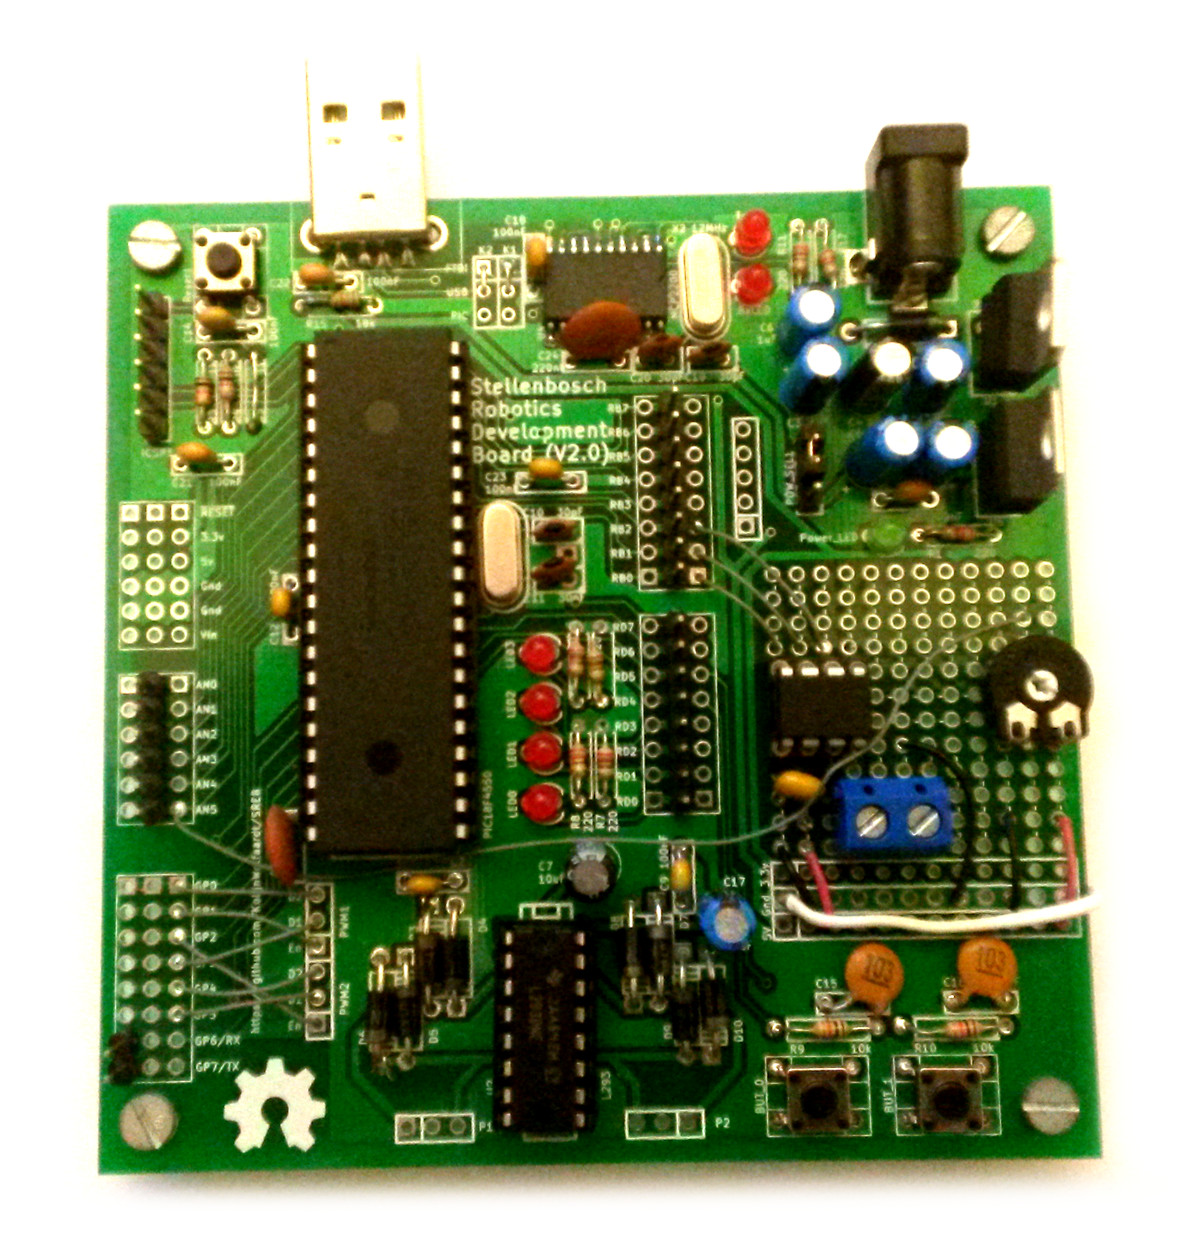
\includegraphics[scale=0.21]{full_board.jpg}
\end{figure}
\section{Hardware}
\subsection{Power Supply}
The main power supply of the board is used to convert battery power to the regulated 5v needed by the PIC. The power input is protected by a diode, to prevent reverse connection. The battery voltage needs to be above 7v to use the board. The protection diode causes a 0.7v drop, and the 7805 regulator requires at least a 6.2v input. Drawing large ammounts of  current from the board will probably cause an additional voltage drop on the battery.

The 5v source for the board is selectable between the battery and the usb. See section \ref{jumper_section} for details. The power led will turn on when the 5v is supplied to the board. The board also contains a 3.3v regulator, should you need 3.3v for any devices.

\subsection{PIC and USB}
The PIC we are using is a PIC18F4550. It is an 8-bit PIC, with a built-in USB module.

\subsection{GPIO Pins}
The GPIO (General purpose input output) pins are laid out in a simmilar fashion as an arduino, but the board is not compatible with arduino shields.

The two banks to the right of the PIC are general purpose pins, and can be used for anything. RD5 to RD0 are used for the LEDs and buttons. You can connect other devices to these lines if you want to, but the buttons/leds will probably no be used then.

The two banks to the left of the pic are power and analog input, respectively. The lowwer bank is usefull for controlling the PWM part of the board. The bottom 2 pins, GP6 and GP7 are used for the UART transmit and receive lines, and should not be used for any other purpose.

Next to the prototyping area there are 3 power rails, one for 5v, one for 0v and a 3.3v rail. There is also another unlabeled power rail, close to the power section. This rail provides V\_in, the input voltage after the protection diode.

\subsection{Motor Driver}
The motor driver is the L298B, and is used to control two motors. It has 6 control inputs, 3 for each motor. The motor driver receives poewr from the battery input, and will only 

\subsection{Buttons and LEDS}

\subsection{Jumpers And configuration}
\label{jumper_section}
\paragraph{Power selection}
There are two important configuration parts on the board. The first is the power select jumper. This allows you to select the 5v power source for the rest of the board. The input can be either the usb connector or the 5v regulated from the battery.
\begin{figure}[h!]
	\centering
    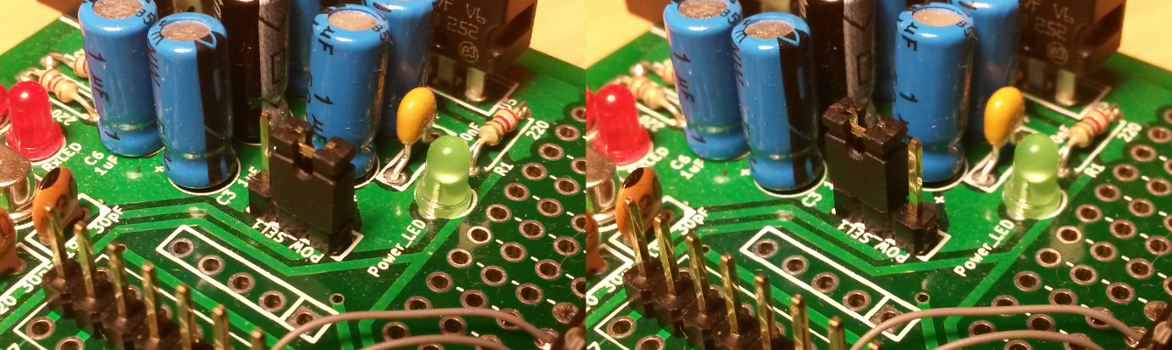
\includegraphics[scale=0.25]{power_jumper.jpg}
    \caption{Left: Power from USB. Right: Power from battery}
\end{figure}

If the usb power is selected you should not try to run high-power devices from the board, such as motors. The motor driver on the board is not poewred from usb. Instead it gets power from the battery input, so it will only work when a battery is connected.


\paragraph{USB data lines}
The usb data lines (D+ and D-) can be redirected between the MCP2200 IC, and the PIC. These should normally be connected to the MCP2200, as this will send the PIC uart to the PC. The PIC has a built in usb module which you can use if you are programming the pic using your own programmer. This can be used to emulate various usb devices, such as keyboards or sound cards. However, this is not easy. The center connection is the usb input, the top connects to the MCP2200, and the bottom to the PIC.
\begin{figure}[h!]
	\centering
    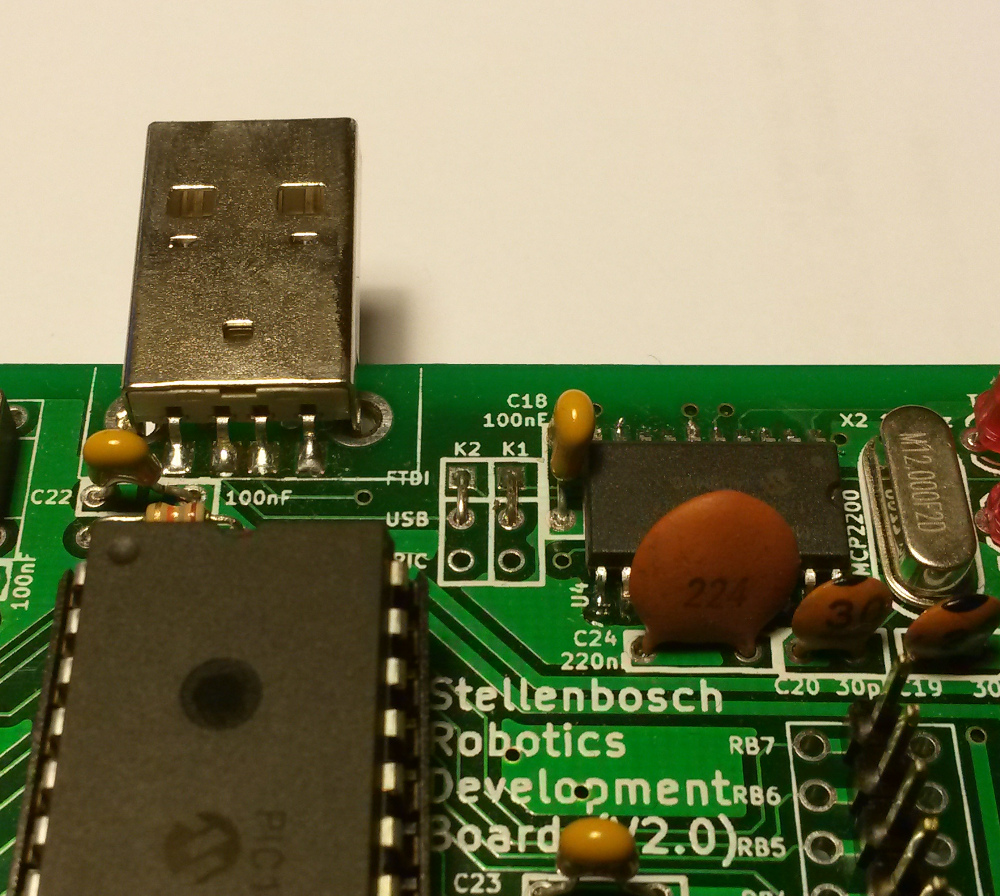
\includegraphics[scale=0.25]{usb_jumpers.jpg}
    \caption {USB connection to usb-UART IC}
\end{figure}

\section {Bootloader}
The bootloader we are using is Tinybootloader \url{http://www.etc.ugal.ro/cchiculita/software/picbootloader.htm} It was written for PICs, with the express goal of occupying very little memory in the PIC.
\paragraph{Basic conecpt}
The bootloader code is written to the PIC, and executes before the main program is run. It detecs if a specific code is sent to it over the UART. If the code is detected within a certain timeout, the bootloader code will start reprogramming the PIC. If the code is not detected, the PIC will continue on to the main program.

\paragraph{Usage}
\begin{enumerate}
\item Select the hex file you want to program to the device. If you compiled using the MPLABX environment, the file might be in one of the build output folders.
\item Select the correct connection settings for the UART. The bootloader uses a 115200 baud rate.
\item Click and hold the reset button on the board. 
\item Click the \textbf{Write Flash} button, and then release the button on the board.
\item The bootloader should now program the device
\end{enumerate}
It is not neccesary to use the \textbf{CheckPIC} button before writing to the PIC.

The program also features a terminal interface, allowing you to send and receive messages from the PIC. An additional feature is the graphing function, which plots the received value as a byte. This is \textit{very} helpfull when debugging sensor outputs. You can transmit the sensor value to the PC, and then whatch the output as you move the sensor. 
\paragraph{On linux}
If you want to use TinyBootloader on linux you will need to run it under \hyperref[Wine]{''http://en.wikipedia.org/wiki/Wine''}, a Linux compatibility layer for Windows. The details of installing and configuring wine will not be discussed here, and some familiarity with linux is assumed.

\begin{enumerate}
  \item To use serial ports, you need to be a member of the dialout group. This group allows you acces to serial ports and modems. To show the groups you are currently added to:

\begin{lstlisting}[language=bash,frame=single]
groups
\end{lstlisting}

If your are not in the dialout group, add yourself using

\begin{lstlisting}[language=bash,frame=single]
sudo adduser username dialout
\end{lstlisting}

To apply the changes you need to log out and log back on.

\item Next you need to find out what device the board registers as. Plug in the board, and run the following command:

\begin{lstlisting}[language=bash,frame=single]
ls /dev
\end{lstlisting}

The device should register as /dev/ttyUSB0 or /dev/ttyACM0

\item You need to tell wine about the device, so add a symbolic link called com1 to the device in the wine configuration folder. The wine configuration might be at a different location depending on your installation. You should also change the destination, the /dev/ttyACM0 part to the device the board registered as.

\begin{lstlisting}[language=bash,frame=single]
ln -s /dev/ttyACM0 ~/.wine/dosdevices/com1 
\end{lstlisting}

\item Now run TinyBootloader in wine. It will not detect the com ports automatically, you will need to enter the com port by hand. After that it should work. Note that if you unplug and replug the board, you will need to restart TinyBootloader.
\end{enumerate}

\section{Writing Code}
\subsection{MPLABX IDE}
The IDE we are using is MPLABX, which is supplied by Microchip. There is an accompaning compiler for the PIC, the XC8 compiler. These can be downloaded from the microchip site, and both work for windows and linux.

\subsection{Skeleton code}


\section{Appendix: Git}
\section{Appendix: Full Schematic}
\end{document}

